\section{Methodology}
\justify
AyurSpace uses a highly decoupled method combining artificial intelligence, mobile
frontend engineering, and backend cloud infrastructure.

\begin{itemize}
    \item \textbf{Presentation Layer (Flutter):}\\
    Built entirely in Flutter; responsible for UI rendering, user input capture,
    localization (ARB files), and cross-platform state updates across Android and iOS.

    \item \textbf{State Management:}\\
    Riverpod is used for reactive state management and DI, isolating UI from business
    logic and enabling components to listen to streams for live changes.

    \item \textbf{Domain Layer (Core Business Logic):}\\
    Pure Dart classes mapping Ayurvedic concepts into technical objects---\texttt{Plant},
    \texttt{Dosha}, \texttt{Remedy}.

    \item \textbf{Plant Taxonomy Integration (Plant.id API):}\\
    User-captured photos are compressed locally then sent to the Plant.id residual
    network for species-level taxonomic classification.

    \item \textbf{LLM Contextualizing (Gemini API):}\\
    After identification, a Chain-of-Thought (CoT) prompt is sent to Gemini, which
    synthesizes Ayurvedic properties: \textit{Rasa}, \textit{Guna}, \textit{Virya},
    and home remedies.

    \item \textbf{Cloud Storage and Authentication:}\\
    Firebase Authentication and Cloud Firestore power secure cross-device synchronization
    of scan history, dosha profiles, and user data.
\end{itemize}

\newpage
\section{Project Plan (Timeline Diagram)}
A Gantt chart illustrates the timeline of project modules from Planning to Deployment.

\setcounter{table}{1}
\begin{table}[!htbp]
\caption{AyurSpace Project Plan}
\label{tab:project_plan}
\centering
\renewcommand{\arraystretch}{1.3}
\begin{tabular}{|c|p{5.5cm}|c|c|c|}
\hline
\textbf{Sr. No} & \textbf{Task Name} & \textbf{Start Date} & \textbf{Finish Date} & \textbf{Duration} \\
\hline
1  & Requirement Analysis          & 01/08/25 & 14/08/25 & 14 days \\
\hline
2  & UI/UX Design                  & 15/08/25 & 04/09/25 & 21 days \\
\hline
3  & System Architecture           & 05/09/25 & 18/09/25 & 14 days \\
\hline
4  & Flutter Setup                 & 20/09/25 & 26/09/25 & 7 days  \\
\hline
5  & Home \& Scan UI               & 27/09/25 & 17/10/25 & 21 days \\
\hline
6  & Chatbot Interface             & 18/10/25 & 31/10/25 & 14 days \\
\hline
7  & Profile \& Settings           & 01/11/25 & 10/11/25 & 10 days \\
\hline
8  & Firebase Auth \& DB           & 15/11/25 & 28/11/25 & 14 days \\
\hline
9  & Plant.id API Integration      & 29/11/25 & 12/12/25 & 14 days \\
\hline
10 & Gemini API Integration        & 13/12/25 & 26/12/25 & 14 days \\
\hline
11 & Unit \& Integration Tests     & 27/12/25 & 16/01/26 & 21 days \\
\hline
12 & User Acceptance Testing       & 17/01/26 & 30/01/26 & 14 days \\
\hline
13 & Bug Fixing \& Polish          & 31/01/26 & 13/02/26 & 14 days \\
\hline
14 & App Store Submission          & 15/02/26 & 21/02/26 & 7 days  \\
\hline
15 & Final Presentation            & 22/02/26 & 26/02/26 & 5 days  \\
\hline
\end{tabular}
\end{table}

\setcounter{figure}{1}
\begin{figure}[!htbp]
\begin{mdframed}
\centering
\resizebox{\linewidth}{!}{%
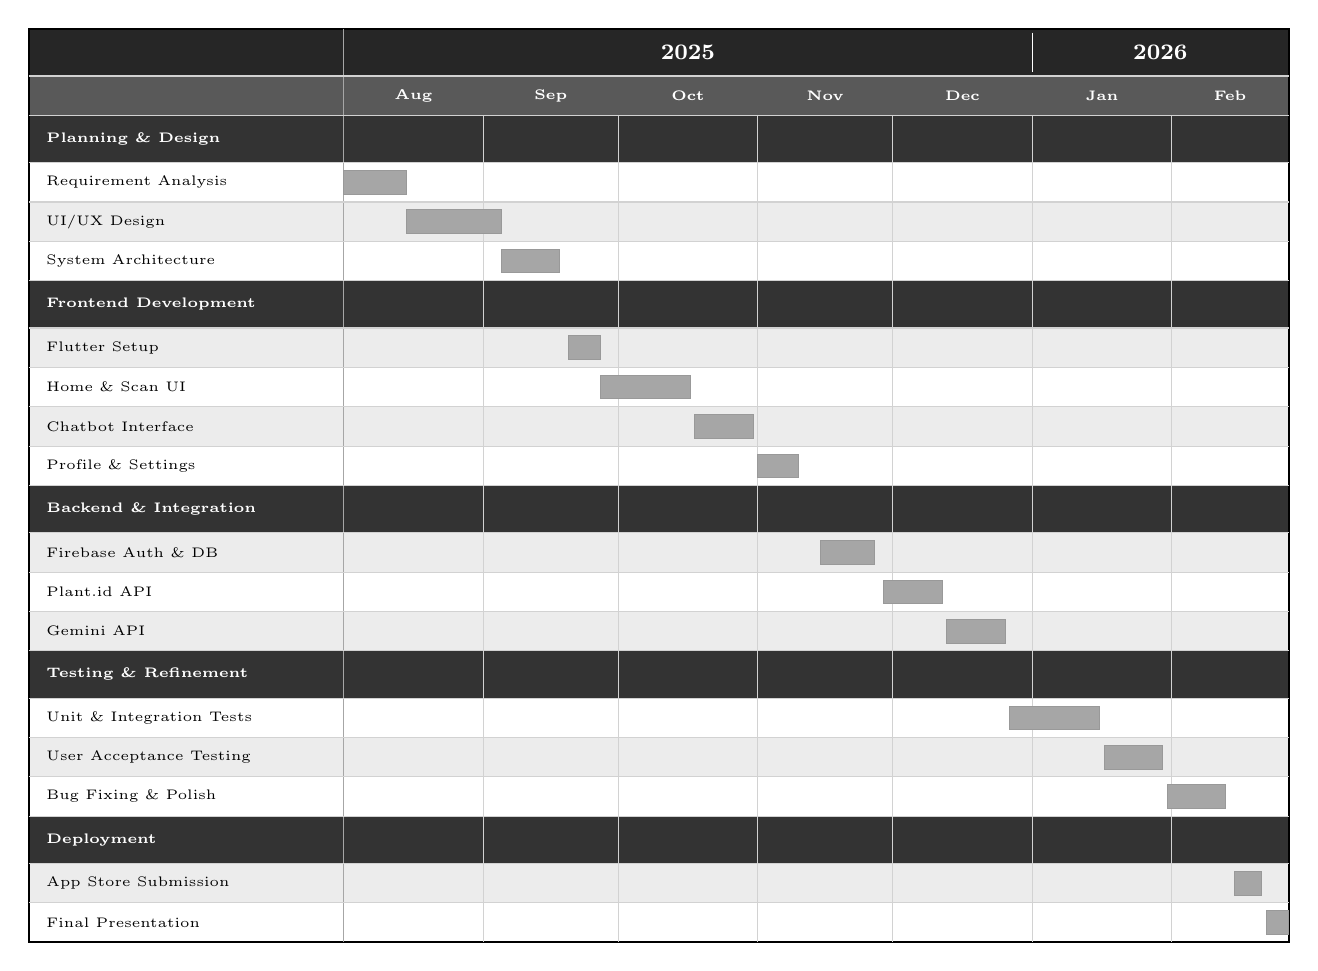
\begin{tikzpicture}[x=1mm, y=1mm]
%%
%% Coordinate system: x=0–160mm (left 40mm = label column, next 120mm = gantt area)
%%                    y=0 (top) down to y=−116mm (bottom)
%% Scale: 120mm / 210 days = 0.5714 mm/day  (Aug 1 = day 0 → x=40)
%% Month x boundaries: Sep1=57.71, Oct1=74.86, Nov1=92.57,
%%                     Dec1=109.71, Jan1=127.43, Feb1=145.14, Feb26=160
%%

%% ── Section header backgrounds ───────────────────────────────────
\fill[black!80] (0,-11)  rectangle (160,-17);
\fill[black!80] (0,-32)  rectangle (160,-38);
\fill[black!80] (0,-58)  rectangle (160,-64);
\fill[black!80] (0,-79)  rectangle (160,-85);
\fill[black!80] (0,-100) rectangle (160,-106);

%% ── Alternating task-row tints ────────────────────────────────────
\fill[gray!15] (0,-22)  rectangle (160,-27);
\fill[gray!15] (0,-38)  rectangle (160,-43);
\fill[gray!15] (0,-48)  rectangle (160,-53);
\fill[gray!15] (0,-64)  rectangle (160,-69);
\fill[gray!15] (0,-74)  rectangle (160,-79);
\fill[gray!15] (0,-90)  rectangle (160,-95);
\fill[gray!15] (0,-106) rectangle (160,-111);

%% ── Year / month header backgrounds ─────────────────────────────
\fill[black!85] (0, 0)  rectangle (160,-6);
\fill[black!65] (0,-6)  rectangle (160,-11);

%% ── Outer border ─────────────────────────────────────────────────
\draw[thick] (0,0) rectangle (160,-116);

%% ── Label | chart separator ──────────────────────────────────────
\draw[gray!70] (40,0) -- (40,-116);

%% ── Month boundary grid lines ────────────────────────────────────
\foreach \x in {57.71, 74.86, 92.57, 109.71, 127.43, 145.14}{
    \draw[gray!35, thin] (\x,-11) -- (\x,-116);
}

%% ── Horizontal row dividers ──────────────────────────────────────
\foreach \y in {-6,-11,-17,-22,-27,-32,-38,-43,-48,-53,
                -58,-64,-69,-74,-79,-85,-90,-95,-100,-106,-111}{
    \draw[gray!35, thin] (0,\y) -- (160,\y);
}

%% ── Year labels ──────────────────────────────────────────────────
\node[white, font=\footnotesize\bfseries] at (83.71,-3)   {2025};
\node[white, font=\footnotesize\bfseries] at (143.71,-3)  {2026};
\draw[white, thin] (127.43,-0.5) -- (127.43,-5.5);

%% ── Month labels ─────────────────────────────────────────────────
\node[white, font=\tiny\bfseries] at (48.86,-8.5)  {Aug};
\node[white, font=\tiny\bfseries] at (66.29,-8.5)  {Sep};
\node[white, font=\tiny\bfseries] at (83.71,-8.5)  {Oct};
\node[white, font=\tiny\bfseries] at (101.14,-8.5) {Nov};
\node[white, font=\tiny\bfseries] at (118.57,-8.5) {Dec};
\node[white, font=\tiny\bfseries] at (136.29,-8.5) {Jan};
\node[white, font=\tiny\bfseries] at (152.57,-8.5) {Feb};

%% ── Section header labels ────────────────────────────────────────
\node[white, font=\tiny\bfseries, anchor=west] at (1,-14)  {Planning \& Design};
\node[white, font=\tiny\bfseries, anchor=west] at (1,-35)  {Frontend Development};
\node[white, font=\tiny\bfseries, anchor=west] at (1,-61)  {Backend \& Integration};
\node[white, font=\tiny\bfseries, anchor=west] at (1,-82)  {Testing \& Refinement};
\node[white, font=\tiny\bfseries, anchor=west] at (1,-103) {Deployment};

%% ── Task labels ──────────────────────────────────────────────────
\node[font=\tiny, anchor=west] at (1,-19.5)  {Requirement Analysis};
\node[font=\tiny, anchor=west] at (1,-24.5)  {UI/UX Design};
\node[font=\tiny, anchor=west] at (1,-29.5)  {System Architecture};
\node[font=\tiny, anchor=west] at (1,-40.5)  {Flutter Setup};
\node[font=\tiny, anchor=west] at (1,-45.5)  {Home \& Scan UI};
\node[font=\tiny, anchor=west] at (1,-50.5)  {Chatbot Interface};
\node[font=\tiny, anchor=west] at (1,-55.5)  {Profile \& Settings};
\node[font=\tiny, anchor=west] at (1,-66.5)  {Firebase Auth \& DB};
\node[font=\tiny, anchor=west] at (1,-71.5)  {Plant.id API};
\node[font=\tiny, anchor=west] at (1,-76.5)  {Gemini API};
\node[font=\tiny, anchor=west] at (1,-87.5)  {Unit \& Integration Tests};
\node[font=\tiny, anchor=west] at (1,-92.5)  {User Acceptance Testing};
\node[font=\tiny, anchor=west] at (1,-97.5)  {Bug Fixing \& Polish};
\node[font=\tiny, anchor=west] at (1,-108.5) {App Store Submission};
\node[font=\tiny, anchor=west] at (1,-113.5) {Final Presentation};

%% ── Task bars  (bar = 3 mm tall, 1 mm padding inside 5 mm row) ───
%% x = 40 + day × 0.5714        (day 0 = Aug 1)

%% Planning & Design
% Requirement Analysis  Aug 01–14  days  0–13  → x 40.00–48.00
\fill[gray!70, draw=gray!80, line width=0.3pt] (40.00,-18) rectangle (48.00,-21);
% UI/UX Design          Aug 15–Sep 04  days 14–34  → x 48.00–60.00
\fill[gray!70, draw=gray!80, line width=0.3pt] (48.00,-23) rectangle (60.00,-26);
% System Architecture   Sep 05–18  days 35–48  → x 60.00–67.43
\fill[gray!70, draw=gray!80, line width=0.3pt] (60.00,-28) rectangle (67.43,-31);

%% Frontend Development
% Flutter Setup         Sep 20–26  days 50–56  → x 68.57–72.57
\fill[gray!70, draw=gray!80, line width=0.3pt] (68.57,-39) rectangle (72.57,-42);
% Home & Scan UI        Sep 27–Oct 17  days 57–77  → x 72.57–84.00
\fill[gray!70, draw=gray!80, line width=0.3pt] (72.57,-44) rectangle (84.00,-47);
% Chatbot Interface     Oct 18–31  days 78–91  → x 84.57–92.00
\fill[gray!70, draw=gray!80, line width=0.3pt] (84.57,-49) rectangle (92.00,-52);
% Profile & Settings    Nov 01–10  days 92–101 → x 92.57–97.71
\fill[gray!70, draw=gray!80, line width=0.3pt] (92.57,-54) rectangle (97.71,-57);

%% Backend & Integration
% Firebase Auth & DB    Nov 15–28  days 106–118 → x 100.57–107.43
\fill[gray!70, draw=gray!80, line width=0.3pt] (100.57,-65) rectangle (107.43,-68);
% Plant.id API          Nov 29–Dec 12  days 120–133 → x 108.57–116.00
\fill[gray!70, draw=gray!80, line width=0.3pt] (108.57,-70) rectangle (116.00,-73);
% Gemini API            Dec 13–26  days 134–147 → x 116.57–124.00
\fill[gray!70, draw=gray!80, line width=0.3pt] (116.57,-75) rectangle (124.00,-78);

%% Testing & Refinement
% Unit & Integration    Dec 27–Jan 16  days 148–168 → x 124.57–136.00
\fill[gray!70, draw=gray!80, line width=0.3pt] (124.57,-86) rectangle (136.00,-89);
% User Acceptance       Jan 17–30  days 169–182 → x 136.57–144.00
\fill[gray!70, draw=gray!80, line width=0.3pt] (136.57,-91) rectangle (144.00,-94);
% Bug Fixing & Polish   Jan 31–Feb 13  days 183–196 → x 144.57–152.00
\fill[gray!70, draw=gray!80, line width=0.3pt] (144.57,-96) rectangle (152.00,-99);

%% Deployment
% App Store Submission  Feb 15–21  days 198–204 → x 153.14–156.57
\fill[gray!70, draw=gray!80, line width=0.3pt] (153.14,-107) rectangle (156.57,-110);
% Final Presentation    Feb 22–26  days 205–209 → x 157.14–160.00
\fill[gray!70, draw=gray!80, line width=0.3pt] (157.14,-112) rectangle (160.00,-115);

\end{tikzpicture}%
}
\end{mdframed}
\caption{Gantt Chart}
\end{figure}

The timeline ensures efficient project management, tracking module initiation and
deadlines for the UI layout, API integration, testing, and deployment phases.

\newpage
\section{Proposed System Architecture}
\justify

\subsection{Layered Architecture}
\begin{enumerate}
    \item \textbf{Presentation Layer}: Flutter --- UI rendering, state updates, user input.
    \item \textbf{Domain Layer}: Core business logic, entities, use-case definitions.
    \item \textbf{Data Layer}: Data retrieval from local caches, Firebase, and third-party APIs.
\end{enumerate}

\subsection{Directory Structure}
\begin{lstlisting}[language=bash]
lib/
|-- config/          # Global configs (API keys, theme, router)
|-- data/            # Models, Repositories, Data Sources
|   |-- models/
|   |-- repositories/
|   |-- sources/
|-- providers/       # Riverpod Providers and Notifiers
|-- screens/         # UI Screens
|-- services/        # Service wrappers (API clients, Firebase)
|-- utils/           # Utilities and helpers
|-- widgets/         # Reusable UI components
\end{lstlisting}

\subsection{Hybrid Neuro-Symbolic Inference Pipeline}
\begin{itemize}
    \item \textbf{Discriminative Phase (Vision)}: Plant.id CNN returns scientific
    classification with confidence score from compressed user image.
    \item \textbf{Generative Phase (Language)}: Scientific name fed to Gemini LLM
    constrained via system prompts to return \textit{Dosha} properties, uses, and
    precautions.
\end{itemize}

\begin{figure}[!htbp]
\begin{mdframed}
  \centering
  \resizebox{0.62\linewidth}{!}{%
  \begin{tikzpicture}[>=Stealth,
      %% ── Base node style ──────────────────────────────────────────
      nd/.style={
          rectangle, rounded corners=10pt, line width=1pt,
          text=white, font=\small\bfseries,
          inner sep=10pt, minimum height=1.5cm,
          text centered, text width=4.0cm
      },
      %% ── Per-layer colors ─────────────────────────────────────────
      usrnd/.style={nd, draw=Teal!50,        fill=Teal!45!black},
      prend/.style={nd, draw=NavyBlue!60,    fill=NavyBlue!70},
      stnd/.style={nd, draw=Orchid!55,       fill=Plum!60!black},
      svcnd/.style={nd, draw=BurntOrange!60, fill=BurntOrange!55!black,
                    text width=3.2cm},
      datnd/.style={nd, draw=ForestGreen!60, fill=ForestGreen!50!black,
                    text width=3.2cm},
      apind/.style={nd, draw=BrickRed!60,    fill=BrickRed!55!black,
                    text width=3.2cm},
      fbsnd/.style={nd, draw=OliveGreen!60,  fill=OliveGreen!50!black,
                    text width=3.2cm},
      %% ── Arrows and labels ────────────────────────────────────────
      arr/.style={-{Stealth[length=7pt,width=5pt]}, thick, draw=black!55},
      lbl/.style={font=\small, fill=white, inner sep=3pt, align=center}
  ]

  %% ─── NODES (top to bottom) ───────────────────────────────────────
  \node[usrnd] (user)  at (0.0, 17.5)
      {Mobile User};
  \node[prend] (pres)  at (0.0, 14.0)
      {Presentation Layer\\[2pt]{\normalfont\footnotesize Flutter Screens}};
  \node[stnd]  (state) at (0.0, 10.6)
      {State Management\\[2pt]{\normalfont\footnotesize Riverpod Providers}};
  \node[svcnd] (svc)   at (-4.0,  7.0)
      {Services Layer\\[2pt]{\normalfont\footnotesize API Wrappers}};
  \node[datnd] (dat)   at ( 4.0,  7.0)
      {Data Layer\\[2pt]{\normalfont\footnotesize Repositories}};
  \node[apind] (api)   at (-4.0,  3.2)
      {External APIs\\[2pt]{\normalfont\footnotesize Plant.id, Gemini}};
  \node[fbsnd] (fbs)   at ( 4.0,  3.2)
      {Firebase Platform\\[2pt]{\normalfont\footnotesize Firestore, Auth}};

  %% ─── CONNECTIONS ─────────────────────────────────────────────────

  %% Mobile User → Presentation Layer
  \draw[arr] (user.south) -- (pres.north);

  %% Presentation Layer → State Management
  \draw[arr] (pres.south) --
      node[lbl, right]{Consumer\\Widget}
      (state.north);

  %% State Management → T-junction → Services + Data
  \coordinate (branch) at (0, 9.1);
  \draw[thick, black!55] (state.south) -- (branch);
  \draw[arr] (branch) -| (svc.north);
  \draw[arr] (branch) -| (dat.north);
  \node[lbl] at (2.2, 9.4) {Repository\\Pattern};

  %% Services Layer → External APIs
  \draw[arr] (svc.south) --
      node[lbl, right]{HTTP REST}
      (api.north);

  %% Data Layer → Firebase Platform
  \draw[arr] (dat.south) --
      node[lbl, right]{Firebase SDK}
      (fbs.north);

  \end{tikzpicture}%
  }
\end{mdframed}
\caption{Proposed System Architecture}
\end{figure}
